\chapter{Interfície d'usuari}

La interfície d'usuari és la part que està més exposada al públic de tot el projecte, ja que serà a través d'on els jugadors de la botifarra viuran les seves experiències i interactuaran amb altres jugadors. Per tal de tenir clar des d'un principi com es volia estructurar es va dissenyar una maqueta de la mateixa abans de començar a treballar. 

\begin{figure}[htbp]
\centering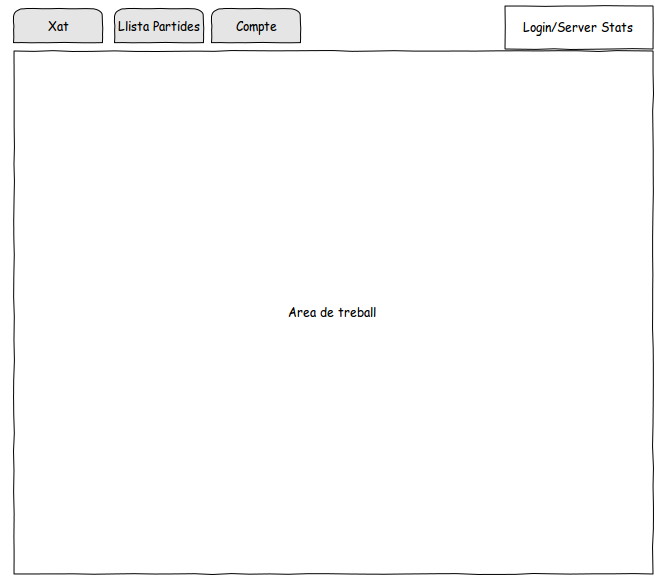
\includegraphics{img/Inici.png}
\caption{Maqueta de la pantalla inicial}
\label{fig:mookup-inici}
\end{figure} 

A la figura \ref{fig:mookup-inici} es pot veure com serà la pantalla inicial. Aquesta s'estructurarà per pestanyes per a que els usuaris puguin accedir a les diferents opcions de la partida. A l'àrea de treball es mostrarà el contingut de les diferents pestanyes. 

\begin{figure}[htbp]
\centering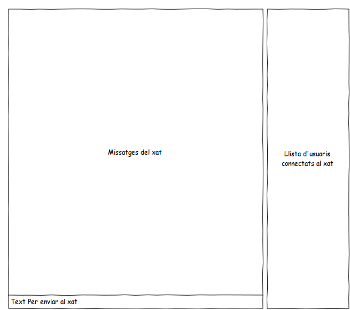
\includegraphics{img/Xat.png}
\caption{Maqueta de la pantalla de Xat}
\label{fig:mookup-xat}
\end{figure} 

A la figura \ref{fig:mookup-xat} es pot veure el contingut que es mostrarà a l'àrea de treball quan la pestanya de xat estigui activa. 

\begin{figure}[htbp]
\centering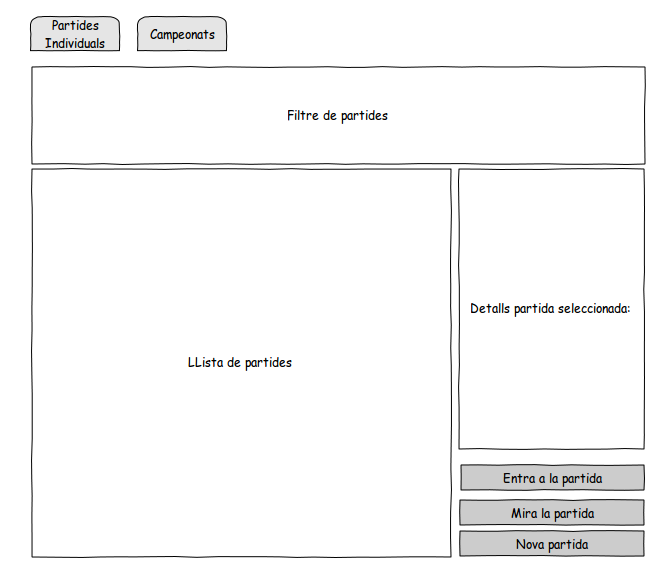
\includegraphics{img/Llista_Partides.png}
\caption{Maqueta del llistat de partides disponibles}
\label{fig:mookup-partides}
\end{figure} 

A la figura \ref{fig:mookup-partides} es pot veure el contingut que es mostrarà a l'àrea de treball quan la pestanya de Llista de partides estigui activa. 

\begin{figure}[htbp]
\centering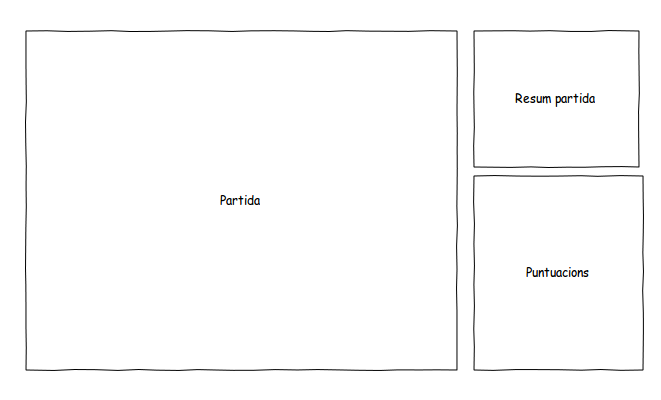
\includegraphics{img/Global_Partida.png}
\caption{Maqueta de la pantalla global de la partida}
\label{fig:mookup-partida}
\end{figure} 

A la figura \ref{fig:mookup-partida} es pot veure el contingut que es mostrarà a l'àrea de treball quan hi hagi una partida en curs. A l'àrea partida serà on els jugadors podran visualitzar el transcurs de la partida i interactuar amb el servidor. Es pot veure en més detall com s'estructura aquesta part en la figura \ref{fig:mookup-detall}.
\begin{figure}[htbp]
\centering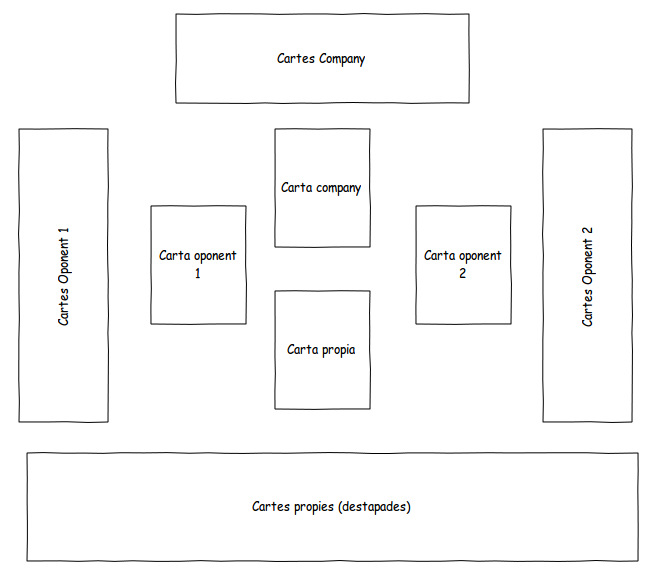
\includegraphics{img/Detall_partida.png}
\caption{Maqueta de la pantalla de detall de la partida}
\label{fig:mookup-detall}
\end{figure} 
